% Task 11: a key from a password. Bob's password and both texts are the answers: question marks.
\documentclass[12pt,tikz,border=6pt]{standalone}
% Shared preamble of the task figures of Lecture 7. The colours are the colour roles of the slides
% (main.tex) and of the passwords simulator:
%   Alice sIndigo, Mallory sPink, message / document / password sViolet, salt sAmber,
%   Bob / the server / the notary sTeal, digest sBrown; mechanisms dark; the unknown: orange dashed.
\usepackage{lmodern}
\usepackage[T1]{fontenc}
\renewcommand{\familydefault}{\sfdefault}
\usepackage{amsmath,amssymb}
\usepackage{xcolor}
\usepackage{fontawesome5}
\usetikzlibrary{arrows.meta, calc, positioning, fit, decorations.pathreplacing, backgrounds}

\definecolor{DeepBlue}{HTML}{283593}
\definecolor{AccentOrange}{HTML}{EB5A14}
\definecolor{nInk}{HTML}{37474F}
\definecolor{nLine}{HTML}{90A4AE}
\definecolor{nLight}{HTML}{CFD8DC}
\definecolor{nFill}{HTML}{ECEFF1}
\definecolor{aExec}{HTML}{43A047}
\definecolor{aWrite}{HTML}{E53935}
\definecolor{sIndigo}{HTML}{5C6BC0}
\definecolor{sPink}{HTML}{EC407A}
\definecolor{sViolet}{HTML}{7E57C2}
\definecolor{sAmber}{HTML}{FFB300}
\definecolor{sTeal}{HTML}{26A69A}
\definecolor{sBrown}{HTML}{8D6E63}
\definecolor{sPinkText}{HTML}{C2185B}
\definecolor{sAmberText}{HTML}{A06A00}
\definecolor{sTealText}{HTML}{00796B}

\tikzset{
  hw/.style={draw=nLine, thick, fill=nFill, text=nInk, rounded corners=3pt, align=center, inner sep=4pt},
  mech/.style={draw=nInk, thick, fill=nInk, text=white, rounded corners=3pt, align=center, inner sep=5pt, font=\small\bfseries},
  msgval/.style={draw=sViolet, thick, fill=sViolet!12, text=nInk, rounded corners=3pt, align=center, inner sep=4pt},
  saltval/.style={draw=sAmber, thick, fill=sAmber!25, text=nInk, rounded corners=3pt, align=center, inner sep=4pt},
  digval/.style={draw=sBrown, thick, fill=sBrown!15, text=nInk, rounded corners=3pt, align=center, inner sep=4pt},
  srvval/.style={draw=sTeal, thick, fill=sTeal!15, text=nInk, rounded corners=3pt, align=center, inner sep=4pt},
  unk/.style={draw=AccentOrange, thick, dashed, fill=white, text=AccentOrange, rounded corners=3pt, align=center,
    inner sep=4pt, font=\bfseries},
  data/.style={-{Stealth}, very thick, nInk},
  person/.style={circle, fill=#1, draw=#1, text=white, minimum size=1.1cm, font=\Large, inner sep=0pt},
}
\newcommand{\personnode}[4]{%
  \node[person=#3] (#1) at (#2) {\faUser};
  \node[font=\small\bfseries, text=#3, below=0.06cm of #1] (#1lbl) {#4};}
\newcommand{\mallorynode}[2]{%
  \node[person=sPink] (#1) at (#2) {\faUserSecret};
  \node[font=\small\bfseries, text=sPinkText, below=0.06cm of #1] (#1lbl) {Mallory};}
\newcommand{\hashbox}[4]{\node[mech, minimum width=#4] (#1) at (#2) {\faCogs\ #3};}

\begin{document}
\pagecolor{white}
\begin{tikzpicture}[>=Stealth]
  \node[font=\small\bfseries, text=nInk, anchor=west] at (-1.0,1.3) {Alice opens her diary};
  \node[msgval, font=\scriptsize\ttfamily] (p) at (0.4,0.4) {violet kettle 1987};
  \node[saltval, font=\scriptsize\ttfamily] (s) at (0.4,-0.4) {salt a3f1094c\ldots};
  \node[mech, minimum width=2.4cm] (k) at (3.6,0) {\faCogs\ PBKDF2\\ \scriptsize 10\,000 iterations};
  \draw[data] (p.east) -- (k); \draw[data] (s.east) -- (k);
  \node[hw, font=\scriptsize, fill=white] (key) at (6.0,0) {\faKey\ key, 32 bytes};
  \draw[data] (k) -- (key);
  \node[mech, minimum width=1.8cm] (c) at (8.4,0) {ChaCha20};
  \draw[data] (key) -- (c);
  \node[hw, font=\scriptsize] (f) at (8.4,1.2) {\faFile*\ diary\_alice.bin};
  \draw[data] (f) -- (c);
  \node[unk, font=\scriptsize] (t) at (11.0,0) {Dear diary, ?};
  \draw[data] (c) -- (t);
  \node[font=\small\bfseries, text=nInk, anchor=west] at (-1.0,-1.5) {Mallory has Bob's diary, not his password};
  \node[circle, fill=sPink, text=white, minimum size=0.9cm, font=\large] (m) at (-0.4,-2.6) {\faUserSecret};
  \node[msgval, font=\scriptsize\ttfamily, text width=1.9cm, align=left] (w) at (1.6,-2.6) {123456\\ password\\ \ldots\\ wordlist.txt};
  \draw[data] (m) -- (w);
  \node[mech, minimum width=2.4cm] (k2) at (4.4,-2.6) {\faCogs\ PBKDF2\\ \scriptsize per guess};
  \draw[data] (w) -- (k2);
  \node[hw, font=\scriptsize] (f2) at (7.0,-1.9) {\faFile*\ diary\_bob.bin};
  \node[mech, minimum width=1.8cm] (c2) at (7.0,-2.9) {ChaCha20};
  \draw[data] (k2) -- (c2); \draw[data] (f2) -- (c2);
  \node[unk, font=\scriptsize, align=left] at (10.6,-2.6) {starts with ``Dear diary,''?\\ password: ?, after ? tries};
\end{tikzpicture}
\end{document}
